\begin{frame}{Obtained Cross Section}
  \begin{figure}
    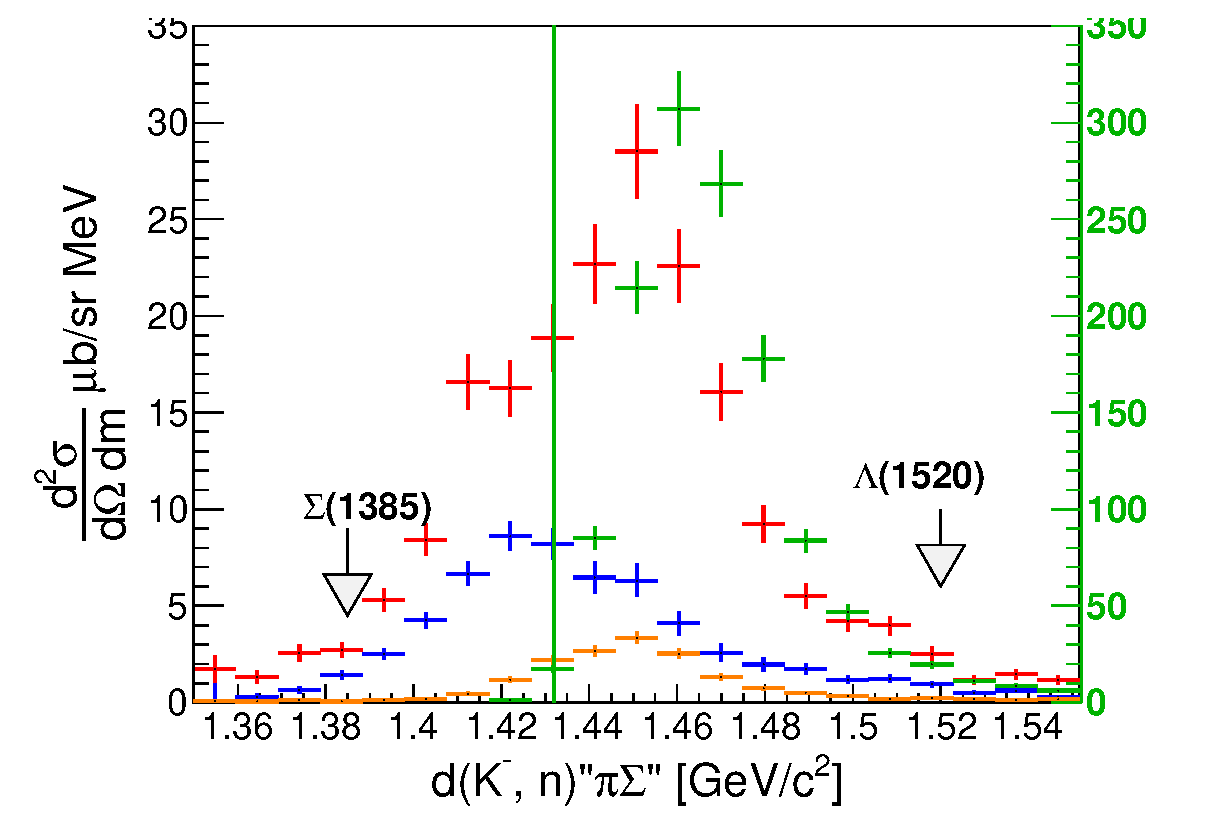
\includegraphics[width=8cm]{../pic/Dron/All_CS.eps}\\
    \footnotesize
    $d(K^-, n)"n K^0"$ is scaled to 1/10.    
  \end{figure}
  \centering
  No structure around $\Sigma(1385)$ ($P-$wave) and $\Lambda(1520)$ ($D-$wave).\\
  $\Rightarrow$ {\bf S-wave dominant.}\\
  $I=0$ ($\pi^-\Sigma^+$ and $\pi^+\Sigma^-$) has excess below the $\bar{K}N$ threshold.
\end{frame}
